\documentclass[]{article}
\usepackage{lmodern}
\usepackage{amssymb,amsmath}
\usepackage{dcolumn} 
\usepackage{ifxetex,ifluatex}
\usepackage{fixltx2e} % provides \textsubscript
\ifnum 0\ifxetex 1\fi\ifluatex 1\fi=0 % if pdftex
  \usepackage[T1]{fontenc}
  \usepackage[utf8]{inputenc}
\else % if luatex or xelatex
  \ifxetex
    \usepackage{mathspec}
  \else
    \usepackage{fontspec}
  \fi
  \defaultfontfeatures{Ligatures=TeX,Scale=MatchLowercase}
\fi
% use upquote if available, for straight quotes in verbatim environments
\IfFileExists{upquote.sty}{\usepackage{upquote}}{}
% use microtype if available
\IfFileExists{microtype.sty}{%
\usepackage{microtype}
\UseMicrotypeSet[protrusion]{basicmath} % disable protrusion for tt fonts
}{}
\usepackage[margin=1in]{geometry}
\usepackage{hyperref}
\hypersetup{unicode=true,
            pdftitle={Concurrent validity of an Estimator of Weekly Alcohol Consumption (EWAC) based on the Extended AUDIT},
            pdfborder={0 0 0},
            breaklinks=true}
\urlstyle{same}  % don't use monospace font for urls
\usepackage[numbers]{natbib}
\bibliographystyle{vancouver}
\usepackage{longtable,booktabs}
\usepackage{graphicx,grffile}
\makeatletter
\def\maxwidth{\ifdim\Gin@nat@width>\linewidth\linewidth\else\Gin@nat@width\fi}
\def\maxheight{\ifdim\Gin@nat@height>\textheight\textheight\else\Gin@nat@height\fi}
\makeatother
% Scale images if necessary, so that they will not overflow the page
% margins by default, and it is still possible to overwrite the defaults
% using explicit options in \includegraphics[width, height, ...]{}
\setkeys{Gin}{width=\maxwidth,height=\maxheight,keepaspectratio}
\IfFileExists{parskip.sty}{%
\usepackage{parskip}
}{% else
\setlength{\parindent}{0pt}
\setlength{\parskip}{6pt plus 2pt minus 1pt}
}
\setlength{\emergencystretch}{3em}  % prevent overfull lines
\providecommand{\tightlist}{%
  \setlength{\itemsep}{0pt}\setlength{\parskip}{0pt}}
\setcounter{secnumdepth}{5}
% Redefines (sub)paragraphs to behave more like sections
\ifx\paragraph\undefined\else
\let\oldparagraph\paragraph
\renewcommand{\paragraph}[1]{\oldparagraph{#1}\mbox{}}
\fi
\ifx\subparagraph\undefined\else
\let\oldsubparagraph\subparagraph
\renewcommand{\subparagraph}[1]{\oldsubparagraph{#1}\mbox{}}
\fi

%%% Use protect on footnotes to avoid problems with footnotes in titles
\let\rmarkdownfootnote\footnote%
\def\footnote{\protect\rmarkdownfootnote}

%%% Change title format to be more compact
\usepackage{titling}

% Create subtitle command for use in maketitle
\providecommand{\subtitle}[1]{
  \posttitle{
    \begin{center}\large#1\end{center}
    }
}

\setlength{\droptitle}{-2em}

  \title{Concurrent validity of an Estimator of Weekly Alcohol Consumption (EWAC)
based on the Extended AUDIT}
    \pretitle{\vspace{\droptitle}\centering\huge}
  \posttitle{\par}
    \author{}
    \preauthor{}\postauthor{}
    \date{}
    \predate{}\postdate{}
  
\usepackage{booktabs}
\usepackage{longtable}
\usepackage{array}
\usepackage{multirow}
\usepackage{wrapfig}
\usepackage{float}
\usepackage{colortbl}
\usepackage{pdflscape}
\usepackage{tabu}
\usepackage{threeparttable}
\usepackage{threeparttablex}
\usepackage[normalem]{ulem}
\usepackage{makecell}
\usepackage{xcolor}

\begin{document}
\maketitle

{
\setcounter{tocdepth}{2}
\tableofcontents
}
\hypertarget{introduction}{%
\section{Introduction}\label{introduction}}

Alcohol consumption is a significant cause of death and ill health. A
number of strategies for prevention \citep{NICE-PH24}, treatment and
harm reduction \citep{NICE-CG115}. Many of those rely on the use of a
screening tool. In the UK, the reference tool is the Alcohol Use
Disorders Identification Test (AUDIT) \citep{Babor2001}, a 10-item
questionnaire schedule widely employed in clinical practice and clinical
research as a diagnostic test for alcohol use disorder (as per
definitions of the International Statistical Classification of Diseases
version 10 F10.1/F10.2; version 11 QE10/6C40.1). The short, 3-item
consumption version known as AUDIT-C has good diagnostics accuracy for
both: (a) interview-based clinical diagnoses; and (b) consumption in
excess of maximum recommended intakes (e.g.~140g/week in Australia, 112
g/week in UK) in a variety of populations \citep{DeMeneses-Gaya2009}.

A variant of the AUDIT-C schedule known as the `Extended AUDIT-C'
improves the granularity of the information collected, thanks to a
greater range of response options on quantity and frequency (items 1 and
2). The Extended AUDIT-C has been used in UK research as part of two
trials \citep{Crane2018, Kaner2013c} and one continuous
household survey \citep{Beard2015a} to capture greater information on
the higher risk drinkers, based on the observation that AUDIT
consumption items are right-truncated.

Neither the AUDIT-C nor the Extended AUDIT-C provide a measure of usual
alcohol consumption, which could help individuals understand, monitor
and adjust their drinking behaviour. Making individuals more aware of
the consumption and associated risk is a key recommendation in the
recent prevention literature \citep{Rehm2016,Nutt2014} and
governmental health recommendations to the public
\citep{AlcoholCMO2016b,AU.alcoguidelines2009}.

The aim of the present study is develop and validate an Estimator of
usual Weekly Alcohol Consumption in units (EWAC) based on the Extended
AUDIT-C. The product of frequency of drinking (AUDIT-C item 1) and
quantity of drinking (AUDIT-C item 2) can be used to estimate usual
alcohol consumption. In addition, measures of heavy use (AUDIT-C item 3)
have been found to improve the consistency of the estimator with other
data sources in previous research \citep{Lemmens1992}.

This paper reports three distinct empirical studies. Study 1 estimates
coefficients to apply to each of the AUDIT-C response items to compute
an EWAC using data from a large English household survey, the Alcohol
Toolkit Study (ATS). It then tests the concurrent validity of the EWAC
across a number of demographic subpopulations in England. Study 2 tests
the contingent validity of the EWAC compared with the 28-day Timeline
Followback in a clinical population (visitors of an acute hospital).
Study 3 compares the population-wide total and empirical cumulative
distribution of alcohol consumption in England using the EWAC, the ATS
graduated frequency schedule, the Health Survey for England, and
official statistics on alcohol sales. The article concludes on the
EWAC's potential applications in research and clinical care.

\hypertarget{methods}{%
\section{Methods}\label{methods}}

\hypertarget{data-sources}{%
\subsection{Data sources}\label{data-sources}}

A longstanding obstacle in alcohol research and care is the absence of a
diagnostic gold standard, which is not addressed even by the development
of new biomarkers. Instead, a number of instruments exist which measure
self-reported alcohol consumption with varying validity and reliability.
A state-of-the art review from \cite{Greenfield2000} is summarised in
\protect\hyperlink{table1}{Table 1} below.

Table 1: Alcohol schedules: selective comparison

\begin{table}[H]
\centering
\begin{tabular}{l|l|l|l}
\hline
Schedule & Bias & Variance & Measures variability\\
\hline
Graduated frequency (GF) & Unclear & Low & Yes\\
Quantity-Frequency (QF) & Unclear & Low & No\\
Quantity-Frequency-Variability (QFV) & Unclear & Low & Yes\\
Yesterday' recall & Minimal & High & No\\
Timeline followback (TLFB) & Low & Low & Yes\\
Prospective diary & Low & Low & Yes\\
\hline
\end{tabular}
\end{table}

Prospective diaries tend to record higher alcohol consumption by
minimising recall bias, followed by GF, while lower levels seem to be
recorded with QF measures \citep{Rehm1998, Heeb2005}.

The present paper employs four sources of data. An overview is available
in \protect\hyperlink{table2}{Table 2} below, together with references
to publicly available methodological descriptions. Analysis of HSE and
ATS microdata was approved by the University of Southampton's Faculty of
Medicine Ethics Committee (ERGO 44682). The hospital questionnaire
(Study 3) collection and analysis was approved by the Health Research
Authority National Research Ethics Service (IRAS 247458; REC
18/SC/0564). All results are reported in UK alcohol units (8g or 10mL of
pure alcohol). Analyses are conducted in \texttt{R}
\citep{RCoreTeam2017} using packages \texttt{tidyverse},
\texttt{survey}, \texttt{rstan}
\citep{package-tidyverse, package-rstan, package-survey, Lumley2004}.
Computer programmes for all analyses are available on an online
repository.

Table 2: Description of data sources

\begin{longtable}[]{@{}lllllrl@{}}
\toprule
\begin{minipage}[b]{0.12\columnwidth}\raggedright
Source\strut
\end{minipage} & \begin{minipage}[b]{0.12\columnwidth}\raggedright
Waves\strut
\end{minipage} & \begin{minipage}[b]{0.12\columnwidth}\raggedright
Population of inference\strut
\end{minipage} & \begin{minipage}[b]{0.12\columnwidth}\raggedright
Alcohol schedules\strut
\end{minipage} & \begin{minipage}[b]{0.12\columnwidth}\raggedright
Validation\strut
\end{minipage} & \begin{minipage}[b]{0.07\columnwidth}\raggedleft
Sample size\strut
\end{minipage} & \begin{minipage}[b]{0.12\columnwidth}\raggedright
Design\strut
\end{minipage}\tabularnewline
\midrule
\endhead
\begin{minipage}[t]{0.12\columnwidth}\raggedright
Alcohol Toolkit Study (ATS) \citep{Beard2015a}\strut
\end{minipage} & \begin{minipage}[t]{0.12\columnwidth}\raggedright
November 2015-October 2017 (waves 110--133)\strut
\end{minipage} & \begin{minipage}[t]{0.12\columnwidth}\raggedright
Residents of private English households aged 16 years and over\strut
\end{minipage} & \begin{minipage}[t]{0.12\columnwidth}\raggedright
Extended AUDIT-C and GF\strut
\end{minipage} & \begin{minipage}[t]{0.12\columnwidth}\raggedright
-\strut
\end{minipage} & \begin{minipage}[t]{0.07\columnwidth}\raggedleft
40,832\strut
\end{minipage} & \begin{minipage}[t]{0.12\columnwidth}\raggedright
TBC\strut
\end{minipage}\tabularnewline
\begin{minipage}[t]{0.12\columnwidth}\raggedright
Health Survey for England (HSE) \citep{NatCenSocialResearch2013}\strut
\end{minipage} & \begin{minipage}[t]{0.12\columnwidth}\raggedright
2011\strut
\end{minipage} & \begin{minipage}[t]{0.12\columnwidth}\raggedright
Residents of private English households aged 18 years and over\strut
\end{minipage} & \begin{minipage}[t]{0.12\columnwidth}\raggedright
Beverage-specific QF\strut
\end{minipage} & \begin{minipage}[t]{0.12\columnwidth}\raggedright
This UK-specific schedule is consistent with a prospective diary
\citep{Boniface2014} and yesterday recall \citep{Stockwell2016}.\strut
\end{minipage} & \begin{minipage}[t]{0.07\columnwidth}\raggedleft
8,610\strut
\end{minipage} & \begin{minipage}[t]{0.12\columnwidth}\raggedright
Multistage random sampling\strut
\end{minipage}\tabularnewline
\begin{minipage}[t]{0.12\columnwidth}\raggedright
Hospital questionnaire study (HOSP)\strut
\end{minipage} & \begin{minipage}[t]{0.12\columnwidth}\raggedright
February 2019 to ??? 2019\strut
\end{minipage} & \begin{minipage}[t]{0.12\columnwidth}\raggedright
Outpatient and day case hospital patients aged 18 years and over\strut
\end{minipage} & \begin{minipage}[t]{0.12\columnwidth}\raggedright
Extended AUDIT-C and TLFB\strut
\end{minipage} & \begin{minipage}[t]{0.12\columnwidth}\raggedright
TLFB records fewer drinking days and thus lower consumption than a
prospective diary \citep{Grant1995}. This recall bias increases with the
\citep{Hoeppner2010, Vinson2003}\strut
\end{minipage} & \begin{minipage}[t]{0.07\columnwidth}\raggedleft
TBC\strut
\end{minipage} & \begin{minipage}[t]{0.12\columnwidth}\raggedright
Cross-sectional recruitment with block randomisation to (a)
self-administered AUDIT-C or (b) researcher-administered AUDIT-C. More
detail in section 2.2.\strut
\end{minipage}\tabularnewline
\begin{minipage}[t]{0.12\columnwidth}\raggedright
Alcohol retail sales \citep{PHE2017}\strut
\end{minipage} & \begin{minipage}[t]{0.12\columnwidth}\raggedright
2014\strut
\end{minipage} & \begin{minipage}[t]{0.12\columnwidth}\raggedright
English population aged 18 years and over\strut
\end{minipage} & \begin{minipage}[t]{0.12\columnwidth}\raggedright
N/A\strut
\end{minipage} & \begin{minipage}[t]{0.12\columnwidth}\raggedright
See \citep{PHE2017}.\strut
\end{minipage} & \begin{minipage}[t]{0.07\columnwidth}\raggedleft
N/A\strut
\end{minipage} & \begin{minipage}[t]{0.12\columnwidth}\raggedright
Ratio of all alcohol produced or processed in the UK, as well as alcohol
imported into the UK for sale and consumption, over the mid-year
population estimate\strut
\end{minipage}\tabularnewline
\bottomrule
\end{longtable}

\hypertarget{study-1-ewac-estimation-and-concurrent-validity}{%
\subsection{Study 1: EWAC estimation and concurrent
validity}\label{study-1-ewac-estimation-and-concurrent-validity}}

A pre-registered protocol for this analysis is available from
\cite{Dutey2018}. We apply methods developed for
quantity-frequency-variability instruments \citep{Lemmens1992} to the
Extended AUDIT-C. For every individual \(i\), we adjusting the product
of \(F_i\) and \(Q_i\) (AUDIT items 1 and 2 respectively) with the
frequency of intense drinking \(V_i\) (AUDIT item 3):

\[\text{EWAC}_i = F_i Q_i + V_ib\]

where \(b\) denotes the average number of units of alcohol consumed in
an intense drinking day. Coefficients \(F, Q, V\) and \(b\) are unknown.
In this study, two sets of potential coefficients are evaluated:

\begin{itemize}
\tightlist
\item
  using the AUDIT response item interval midpoint: for example, 2.5 for
  `2 to 3 times per week' in AUDIT item 2
\item
  using a statistical model to estimate the coefficients directly from
  the ATS (further detail in supplementary material).
\end{itemize}

The ATS data is affected by missing data: 35.3\% of respondents (14,408)
reported never drinking alcohol in AUDIT item 1 and were not asks any
further AUDIT or GF questions.\footnote{Note: Data from HSE on
  `never-never?' indicates that a third are probably occasional
  drinkers. Consider adding the diagram previously drawn for ABH} They
were thus excluded from the analysis. A further 4,020 respondents (0.2\%
of those reporting drinking in AUDIT item 1) did not have a valid GF
alcohol consumption record and were also excluded. Missing data in the
ATS' GF schedule is assumed to be missing at random conditionally on the
Extended AUDIT-C responses.

The discrepancy between the EWAC and the GF schedule is quantified, by
treating GF as a gold standard. It enables the examination of two types
of deviations across every participant \(i\) in the ATS sample:

\begin{itemize}
\tightlist
\item
  MD: the mean deviation
  \(\sum_{i=1}^{n}{n^{-1}(\rm{EWAC_i} - \rm{GF_i} )}\) can be
  assimilated to a measure of bias under the assumption that GF is a
  gold standard.
\item
  RMSD: the root mean squared deviation
  \(\sum_{i}{\sqrt{( \rm{EWAC_i} - \rm{GF_i} )^2}}\) can be assimilated
  to a measure of total error: it capture both bias and random deviation
  from the assumed gold standard.
\end{itemize}

We test the hypothesis that the EWAC's validity varies across population
subgroups by regressing both (a) the simple deviation and (b) the root
squared deviation in linear regression models, against the following
predictors: sex by age group; ethnic group; favourite drink (wine, beer,
etc.); highest educational qualification; religion; smoking status;
general health; recent attempts at reducing or stopping drinking.

\hypertarget{study-2-concurrent-validity-in-hospital-outpatients}{%
\subsection{Study 2: Concurrent validity in hospital
outpatients}\label{study-2-concurrent-validity-in-hospital-outpatients}}

A second study aims to confirm the robustness of findings in (a)
healthcare patients; (b) when the Extended AUDIT-C; (c) and against
another alcohol schedule than GF. The latter aim is justified by the
absence of undisputed diagnostic gold standard for alcohol consumption.
To this end, participants were recruited from a range of clinics at a
large acute hospital in Southampton, UK: orthopaedics outpatient,
endoscopy day cases, young adult outpatient, infusion ???. Participants
were first randomised to one of two groups: (1) self-administered
Extended AUDIT-C and (2) researcher-administered Extended AUDIT-C using
block randomisation. Once this questionnaire completed, both groups were
asked to complete a 28-day Alcohol TFLB questionnaire administered by
the researcher.

Sample size was set to power three statistical hypotheses listed in
\cite{Dutey2018}. An internal pilot conducted on 130 participants was
used to obtain estimates of the variance in MD. The study was powered to
detect a minimum MD between EWAC and TLFB of 1 unit. Using a two-sided
paired \emph{t}-test, 80\% power and 95\% confidence, the required
sample size was 387 in total. In addition, the study was powered to
detect a minimum RMSD greater than \(\text{RMSD}_{H_0} = 2\) units using
a one-sided, one-sample \(\chi^2\) test of variance. This involves
testing the null hypothesis, \(H_0: \text{RMSD}^2 = 4\) versus the
one-sided alternative hypothesis \(H_a: \text{RMSD}^2 > 4\). Dixon \&
Massey \citep{Dixon1983} set the minimum detectable value of the
variance as
\(\text{RMSD}_{H_a}^2 = \text{RMSD}_{H_0}^2 . \chi^2_{n-1, 1-\alpha} / \chi^2_{n-1, 1-\beta}\).
With \(n = 130\), \(\alpha = 0.05\) and \(\beta=.2\),
\(\text{RMSD}_{H_a} = 2.37\). The test statistic
\(\chi^2 = (n-1)\text{RMSD}^2 / 4\) follows a \(\chi^2\) distribution
with \(n-1\) degrees of freedom. The normal approximation proposed by
Dixon \& Massey \citep{Dixon1983} to the sample size require is
\[n = 1/2 \left( \dfrac{z_{1-\alpha}-z_\beta}{\ln(\text{RMSD}_{H_a}) - \ln(\text{RMSD}_{H_0})}\right)^2  \]

In our pilot study, the required sample size was 106, that is inferior
to the target pilot sample size.

To model the relationship between the EWAC and the TLFB, the number of
units consumed on any day was assumed to follow a Poisson distribution,
the rate of which is determined by the latent usual alcohol consumption
as well as the following variables: AUDIT mode of administration
(self-administered; researcher-administered), week day, number of days
elapsed since (1-7; 8-14; 15-21; 22-28). TLFB daily number of units
consumed were rounded to the nearest integer and regressed in a Poisson
regression model against the aforementioned predictor, as well as the
EWAC divided by 7 to obtain its daily equivalent. The corresponding
regression coefficient measures the ratio of TLFB to EWAC.

\hypertarget{study-3-aggregate-concurrent-validity}{%
\subsection{Study 3: Aggregate concurrent
validity}\label{study-3-aggregate-concurrent-validity}}

We examine the aggregate consistency in alcohol consumption estimates
across all residents of England aged 18 years and over by plotting the
empirical cumulative distribution of alcohol consumption given by (1)
the EWAC estimated from the ATS; (2) the quantity-frequency estimated in
the ATS; (3) the beverage-specific estimators in HSE in 2011; (4) the
prospective diary estimator in HSE 2011. In this analysis, survey
weights are used: in (1-3), poststratification weights estimated using
calibration and age-sex MYPES; in (4), similar postratification weights
adjusted for self-selection into participation to the prospective diary
data collection. Finally, we examine the percentage of total alcohol
sales for England accounted for by each method. Alcohol sales (both
on-trade and off-trade) estimates for England (population aged 18 years
and over) in 2014 were obtained from Public Health England
\citep{PHE2017}.

\hypertarget{results}{%
\section{Results}\label{results}}

\hypertarget{study-1-ewac-estimation-and-validation}{%
\subsection{Study 1: EWAC estimation and
validation}\label{study-1-ewac-estimation-and-validation}}

\hypertarget{ewac-coefficients}{%
\subsubsection{EWAC coefficients}\label{ewac-coefficients}}

The first step involved choosing a set of coefficients to compute the
EWAC. We compare using the midpoint of the AUDIT item intervals; and
coefficients estimated using a statistical model. The EWAC based on
midpoint coeffients produces a mean deviation (MD) of 0.71 alcohol units
(\(p\) \textless{} 0.001), suggesting a slight positive bias. The root
mean squared deviation (RMSD) is estimated at 12.28, significantly
grater than 4 (\(p\) \textless{} 0.001), suggesting that the EWAC of any
given individual would be on average 12 units from the truth (treating
GF schedule can be used as a gold-standard).

Coefficients estimated by the statistical model provide a small
improvement, but bias remains statistically significant with MD = 0.18
(\(p\) = 0.012). Error remains statistically significantly greater than
4 with RMSD = 10.94 (\(p\) \textless{} 0.001).
\protect\hyperlink{figure1}{Figure 1} compares individual EWAC and GF
values. We note the departure of lines of best fit from the diagonal,
whether estimated using ordinary least squares or using a thin plate
regression spline. This is an indication that the EWAC is consistently
lower than GF, even with coefficients estimated from the statistical
model on the same data source. This discrepancy is noticeable for high
levels of consumption (at least 30 units per week).


\includegraphics[width = .5\linewidth]{analysis_files/figure-latex/unnamed-chunk-3-1.pdf} 
\includegraphics[width = .5\linewidth]{analysis_files/figure-latex/unnamed-chunk-4-1.pdf}

Figure 1: Plot of EWAC against GF in ATS with ordinary least square
regression line (\(n\) = 22,373)

\hypertarget{heterogeneous-error}{%
\subsubsection{Heterogeneous error}\label{heterogeneous-error}}

Next, the MD and RMSD are regressed against respondents characteristics
in order to identify subgroups with potentially stronger bias or error
(\protect\hyperlink{tab_ewac_validity_reg}{Table 3}). \(R^2\) statistics
suggest that the factors account for a very modest proportion of both MD
and RMSD (\textless{}2\%). Despite this:

\begin{itemize}
\tightlist
\item
  MD is 4.8 units {[}2.1, 7.5{]} with in Black respondents and 5.9 units
  {[}1.6, 10.2{]} higher in respondents from Black and Other ethnic
  groups respectively, while RMSD not significantly different from the
  rest of the population. This suggests EWAC has a strong positive bias
  in Black respondents.
\item
  RMSD is reduced by an average 2 units with an educational
  qualification compared to no qualifications, without effect on MD
\item
  MD is reduced by 1.1 units {[}0.4, 1.8{]}, while RMSD is increased by
  2.5 units {[}1.8, 3.1{]} in current smokers compared with
  never-smokers.
\end{itemize}

There was no evidence of properties of the EWAC being different across
gender and age groups.

 
\begin{table}[!htbp] \centering 
	\caption{Coefficients of linear regression of the bias and error of EWAC
		compared with GF}
\begin{tabular}{@{\extracolsep{5pt}}lD{.}{.}{-1} D{.}{.}{-1} } 
\\[-1.8ex]\hline 
\hline \\[-1.8ex] 
\\[-1.8ex] & \multicolumn{1}{c}{MD} & \multicolumn{1}{c}{RMSD} \\ 
\hline \\[-1.8ex] 
 Constant & 2.9$ $(-8.8$, $14.5) & 4.0$ $(-5.8$, $13.8) \\ 
  sexMen & -0.4$ $(-14.7$, $14.0) & 0.6$ $(-11.5$, $12.7) \\ 
  ageg18-24 years & -1.5$ $(-13.1$, $10.1) & 2.7$ $(-7.1$, $12.5) \\ 
  ageg25-34 years & -2.5$ $(-14.1$, $9.1) & 2.6$ $(-7.2$, $12.4) \\ 
  ageg35-44 years & -3.3$ $(-14.9$, $8.4) & 4.0$ $(-5.8$, $13.8) \\ 
  ageg45-54 years & -2.0$ $(-13.6$, $9.7) & 3.6$ $(-6.2$, $13.3) \\ 
  ageg55-64 years & -0.3$ $(-11.9$, $11.4) & 4.2$ $(-5.6$, $14.0) \\ 
  ageg65-74 years & -1.1$ $(-12.8$, $10.6) & 4.3$ $(-5.5$, $14.1) \\ 
  ageg75-84 years & 1.1$ $(-11.0$, $13.1) & 4.5$ $(-5.6$, $14.7) \\ 
  ageg85+ years & 5.0$ $(-8.7$, $18.6) & 8.3$ $(-3.2$, $19.9) \\ 
  ethgrpWhite Other & 1.6$ $(0.2$, $3.0)^{*} & -0.00$ $(-1.2$, $1.2) \\ 
  ethgrpMixed & -1.5$ $(-4.1$, $1.0) & 0.9$ $(-1.3$, $3.0) \\ 
  ethgrpAsian & 2.4$ $(-0.5$, $5.3) & -1.3$ $(-3.8$, $1.1) \\ 
  ethgrpBlack & 4.8$ $(2.1$, $7.5)^{***} & 1.5$ $(-0.8$, $3.8) \\ 
  ethgrpOther & 5.9$ $(1.6$, $10.2)^{**} & -0.3$ $(-3.9$, $3.3) \\ 
  favdrinkCider & -1.1$ $(-2.5$, $0.2) & 1.1$ $(-0.1$, $2.2) \\ 
  favdrinkMixed spirits & 1.3$ $(-0.1$, $2.6) & -1.2$ $(-2.3$, $-0.1)^{*} \\ 
  favdrinkOther & 3.5$ $(-0.1$, $7.0) & -1.4$ $(-4.4$, $1.6) \\ 
  favdrinkSpirits alone & 1.0$ $(-0.1$, $2.1) & 0.9$ $(-0.1$, $1.8) \\ 
  favdrinkWine & 0.7$ $(-0.1$, $1.4) & -0.6$ $(-1.3$, $-0.01)^{*} \\
 Attempt to cut down& & \\
 
   in last 12 months & -0.5$ $(-1.2$, $0.1) & 1.6$ $(1.1$, $2.2)^{***} \\ 
  religionChristian & 0.2$ $(-0.4$, $0.8) & -0.1$ $(-0.6$, $0.4) \\ 
  religionMuslim & 4.6$ $(-4.7$, $13.9) & 3.9$ $(-4.0$, $11.7) \\ 
  religionAny other religion & -1.7$ $(-3.4$, $-0.01)^{*} & 2.8$ $(1.4$, $4.2)^{***} \\ 
  highqualNVQ \textless = 3 & 0.2$ $(-0.9$, $1.4) & -1.7$ $(-2.7$, $-0.7)^{***} \\ 
  highqualNVQ4+ (degree) & 0.1$ $(-1.2$, $1.3) & -2.6$ $(-3.6$, $-1.5)^{***} \\ 
  highqualOther & -0.8$ $(-2.4$, $0.7) & -2.0$ $(-3.3$, $-0.7)^{**} \\ 
  smokstatStopped\textgreater 1y ago & -0.6$ $(-1.3$, $0.2) & 0.5$ $(-0.1$, $1.1) \\ 
  smokstatStopped in past year & -0.5$ $(-2.6$, $1.6) & 1.0$ $(-0.8$, $2.7) \\ 
  smokstatSmoker & -1.1$ $(-1.8$, $-0.4)^{**} & 2.5$ $(1.8$, $3.1)^{***} \\ 
  sexMen:ageg18-24 years & -1.1$ $(-15.5$, $13.4) & 1.3$ $(-10.9$, $13.4) \\ 
  sexMen:ageg25-34 years & -0.9$ $(-15.4$, $13.5) & 0.9$ $(-11.3$, $13.0) \\ 
  sexMen:ageg35-44 years & -1.0$ $(-15.5$, $13.4) & 0.8$ $(-11.4$, $13.0) \\ 
  sexMen:ageg45-54 years & -1.8$ $(-16.3$, $12.6) & 1.1$ $(-11.1$, $13.2) \\ 
  sexMen:ageg55-64 years & -2.1$ $(-16.5$, $12.4) & 1.0$ $(-11.2$, $13.2) \\ 
  sexMen:ageg65-74 years & 0.4$ $(-14.1$, $14.9) & 1.1$ $(-11.1$, $13.3) \\ 
  sexMen:ageg75-84 years & -1.5$ $(-16.3$, $13.4) & -0.7$ $(-13.2$, $11.8) \\ 
  sexMen:ageg85+ years & -7.3$ $(-23.9$, $9.3) & -1.0$ $(-15.0$, $13.0) \\ 
 Observations & \multicolumn{1}{c}{9,850} & \multicolumn{1}{c}{9,850} \\ 
R$^{2}$ & \multicolumn{1}{c}{0.02} & \multicolumn{1}{c}{0.03} \\ 
Adjusted R$^{2}$ & \multicolumn{1}{c}{0.01} & \multicolumn{1}{c}{0.02} \\ 
Residual Std. Error (df = 9812) & \multicolumn{1}{c}{14.4} & \multicolumn{1}{c}{12.1} \\ 
F Statistic (df = 37; 9812) & \multicolumn{1}{c}{4.4$^{***}$} & \multicolumn{1}{c}{7.1$^{***}$} \\ 
\hline \\[-1.8ex] 
\textit{Notes:} & \multicolumn{2}{l}{$^{*}$P $<$ .05} \\ 
 & \multicolumn{2}{l}{$^{**}$P $<$ .01} \\ 
 & \multicolumn{2}{l}{$^{***}$P $<$ .001} \\ 
\end{tabular} 
\end{table}

\hypertarget{study-2-concurrent-validity-in-hospital-patients}{%
\subsection{Study 2: Concurrent validity in hospital
patients}\label{study-2-concurrent-validity-in-hospital-patients}}

A total of 130 participants were recruited in hospital clinics, with
data successfully collected on the Extended AUDIT-C for 81\% of
participants (\(n\) = 105) at baseline. The Extended AUDIT-C was
administered first, with 44 participants randomised to
self-administration using a pen and paper form, while the remaining 61
were administered by a researcher.

\begin{table}[!htbp] \centering 
  \caption{Coefficients of regression of TLFB daily consumption against
  	EWAC, administration of the week, week day and time} 
  \label{} 
\begin{tabular}{@{\extracolsep{5pt}}lD{.}{.}{-1} } 
\\[-1.8ex]\hline 
\hline \\[-1.8ex] 
\\[-1.8ex] & \multicolumn{1}{c}{TFLB} \\ 
\hline \\[-1.8ex] 
 Constant & -0.5$ $(-0.6$, $-0.3)^{***} \\ 
  ewac\_stan\_log & 1.1$ $(1.1$, $1.2)^{***} \\ 
  q\_admin\_modeSelf & 0.1$ $(-0.01$, $0.2) \\ 
  week\_since8-14 days & -0.1$ $(-0.2$, $-0.01)^{*} \\ 
  week\_since15-21 days & -0.04$ $(-0.1$, $0.1) \\ 
  week\_since22-28 days & -0.1$ $(-0.2$, $0.04) \\ 
  tlfb\_weekdayMonday & -0.01$ $(-0.2$, $0.2) \\ 
  tlfb\_weekdayTuesday & 0.2$ $(0.02$, $0.4)^{*} \\ 
  tlfb\_weekdayWednesday & 0.1$ $(-0.1$, $0.3) \\ 
  tlfb\_weekdayThursday & 0.7$ $(0.6$, $0.9)^{***} \\ 
  tlfb\_weekdayFriday & 1.3$ $(1.1$, $1.4)^{***} \\ 
  tlfb\_weekdaySaturday & 0.6$ $(0.4$, $0.7)^{***} \\ 
 Observations & \multicolumn{1}{c}{2,803} \\ 
Log Likelihood & \multicolumn{1}{c}{-4,322.8} \\ 
Akaike Inf. Crit. & \multicolumn{1}{c}{8,669.6} \\ 
\hline \\[-1.8ex] 
\textit{Notes:} & \multicolumn{1}{l}{$^{*}$P $<$ .05} \\ 
 & \multicolumn{1}{l}{$^{**}$P $<$ .01} \\ 
 & \multicolumn{1}{l}{$^{***}$P $<$ .001} \\ 
\end{tabular} 
\end{table}

To estimate comparable measures of deviaiton as in previous sections,
the model is used to impute the 137 out of 105 daily consumption figures
that were missing in total for 13 participants. In this small pilot
dataset, MD = -0.7 unit is measured (\(p\) = 0.199) while RMSD = 5.3 and
is statistically significantly greater than 2 units (\(p\) \textless{}
0.001)



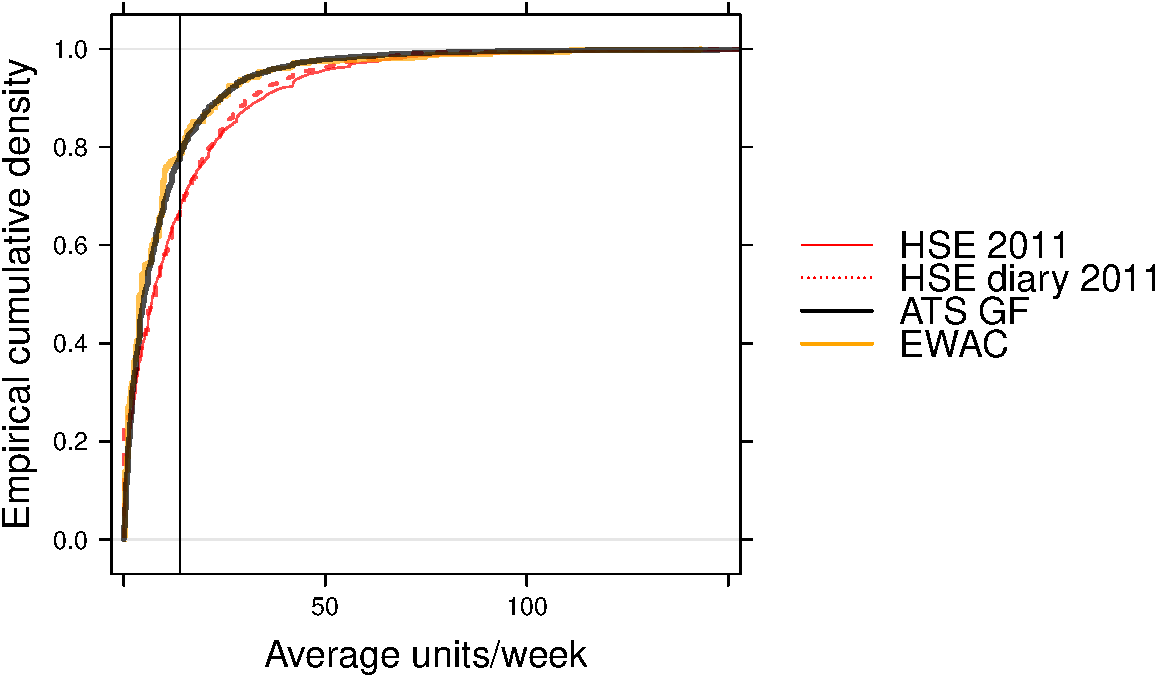
\includegraphics[width=.8\linewidth]{analysis_files/figure-latex/unnamed-chunk-8-1.pdf}

Figure 2: Plot of EWAC estimates against TLFB estimates in hospital
participants with lines of fit


\hypertarget{study-3-empirical-distribution-functions}{%
\subsection{Study 3: Empirical distribution
functions}\label{study-3-empirical-distribution-functions}}

Table 5 provides estimates of total alcohol consumption in adult
resident of private households in England using four different
estimators, and compares them with alcohol retail sales. The HSE
schedules provide the highest estimates of alcohol consumption and
coverage of sale statistics. The proposed EWAC estimates of total
consumption are just 77\% of a very reliable estimate, the HSE
prospective diary. \textbf{ADD YESTERDAY METHOD!}

Figure 3 suggests that the EWAC, like the ATS GF it was estimated
against, estimates a higher prevalence of low risk consumption
(\textless{}= 14 units/week) and increased risk consumption than HSE. In
constrast very high alcohol consumption (\textgreater{}= 50 units/week)
is higher in HSE. This may be due to a combination of difference in
sampling coverage, nonresponse bias, or measurement error in the alcohol
schedules.

Table 5: Summary statistics on alcohol consumption in England in
residents aged 18 years and over (excluding abstainers)

\begin{longtable}[]{@{}lrrrrr@{}}
\toprule
Study & Mean (units/week) & Median & Variance & N & \% of alcohol
sold\tabularnewline
\midrule
\endhead
HSE beverage-specific QF & 14.0 & 7.3 & 474.6 & 6,545 &
72.4\tabularnewline
HSE prospective diary & 12.7 & 8.0 & 264.7 & 4,640 & 66.0\tabularnewline
ATS GF & 10.0 & 5.1 & 242.0 & 22,136 & 51.9\tabularnewline
ATS EWAC & 9.8 & 4.4 & 245.0 & 25,882 & 50.9\tabularnewline
Retail sales & 19.3 & -- & -- & -- & --\tabularnewline
\bottomrule
\end{longtable}



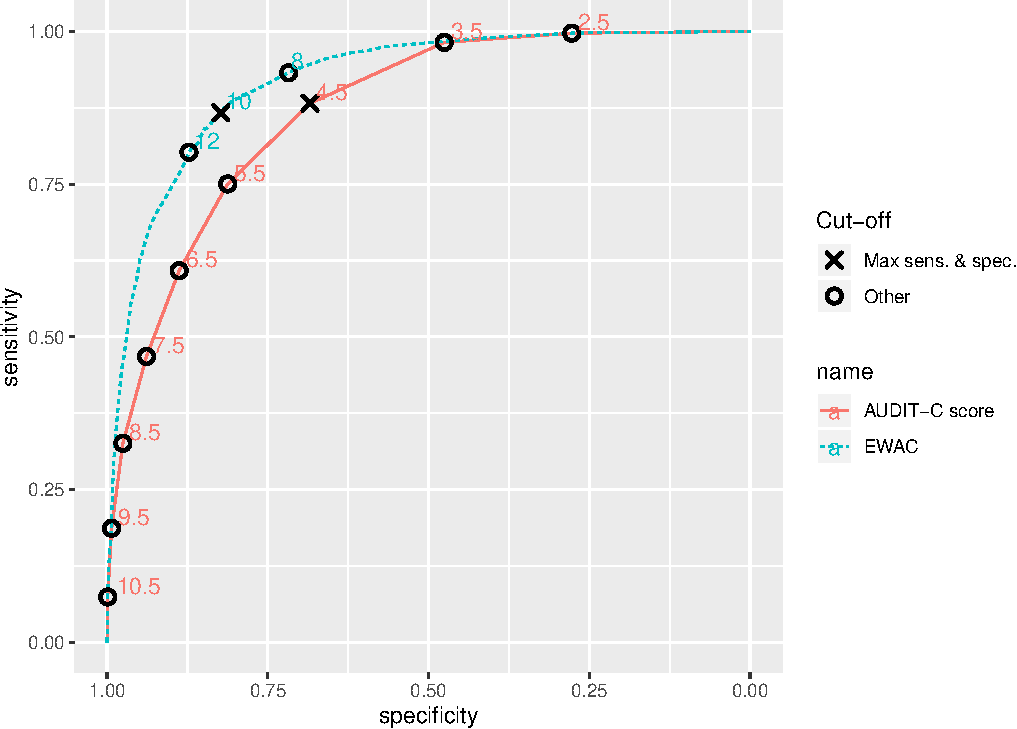
\includegraphics{analysis_files/figure-latex/unnamed-chunk-11-1.pdf}

Figure 3: Empirical cumulative distribution function of weekly alcohol
consumption in England according to four alcohol schedules in residents
aged 18 years and over

\hypertarget{discussion}{%
\section{Discussion}\label{discussion}}

\hypertarget{main-findings}{%
\subsection{Main findings}\label{main-findings}}

To the best of our knowledge, this is the first paper to develop an EWAC
using a well-accepted and fast alcohol questionnaire such as the AUDIT.
We used the Extended AUDIT-C to address the AUDIT-C's right-truncation
and estimate consumption even for heavy consumers.

We find that it is possible to provide an EWAC with a margin of error of
XX units using gender-specific coefficients, with consistent results
across the English population.

Much like we produced gender-specific coefficients, it would be possible
to use age information to adjust coefficients. is consitent with
previous research suggesting largest discrepancy is noted for
individuals aged 85 years and over

Knowledge of alcohol beverage content remains insufficient in the UK. In
the 2007 HSE, just 31\% of frequent beer drinkers and 17\% of frequent
wine drinkers were not aware of the unit equivalence to their intake.
These proportions were found to be even lower in all other drinkers.

This study reports an extensive range of validation analyses on the
EWAC's validity and reliability. Findings are valid for the general
population of England, although they may not generalise to other
populations excluded from our sampling frames, such as residents of
communal and carceral institutions, homeless people, or migrant
populations. Similarly, findings may not designated to small
subpopulations with an atypical alcohol consumption, such as patients
seeking care for conditions such as addition or alcohol liver disease.

\hypertarget{limitations}{%
\subsection{Limitations}\label{limitations}}

As noted previously, a low proportion of the population knows the
alcohol content of what they drink in units. This may influence the
reliability of AUDIT item 2 (quantity), particularly in cases when it is
self-administered or administered without guidance on beverage alcohol
content. In this paper, the AUDIT scheduled was administered by a
researcher in all cases but XXX participants in study 3; and even those
were given a showcard summarising the unit content of most popular
beverages.

respondents who drank beer and those who drank wine at least once a week
were much more likely to know how many units were in that drink than
were those who seldom drank these drinks, but even so, a of the

drinking diary was given to all participants aged 18 and over who
completed the main HSE interview and had had an alcoholic drink in the
previous 12 months.

\hypertarget{is-the-ewac-good-enough-to-be-used}{%
\subsection{Is the EWAC good enough to be
used?}\label{is-the-ewac-good-enough-to-be-used}}

Our findings demonstrate that the mean deviation between EWAC and a more
time-consuming alcohol schedule is XX (GF) and XX (TFLB). In other
words, 95\% of respondents' expected alcohol intake may be up to X units
away from the EWAC. Other clinical parameters may be affected by similar
uncertainty. For instance, blood pressure is highly variables and can be
xx off using a single reading. Specific patient and public involvement
is needed to understand how satisfactory this precision is. In the
meantime, we argue that the EWAC can be useful to both clinicians and
patients alongside established AUDIT-C thresholds: it can be used to
engage a conversation around health risks of alcohol and recommendations
to maintain consumption below 14 units in the UK. We also think it can
be less stigmatising than a score in excess of 5, which can often be
interpreted by patients as being labelled as alcohol dependent or
problem drinker.

\hypertarget{what-are-the-potential-applications}{%
\subsection{What are the potential
applications?}\label{what-are-the-potential-applications}}

Important contributions by Nutt and Rehm invite us to reconsider alcohol
care practice in favour of a more clinical approach. These authors argue
that alcohol consumption should be treated like any other risk factor:
blood pressure or cholesterol are frequently monitored by general
physicians in a non stigmatising way and managed as well as possible.
Similarly, Rehm and Nutt's view is that individuals should know their
consumption, and general practitioners should be able to engage with
patients effectively in managing risks. Where lifestyle interventions
are unsuccessful, pharmacological alternatives should be sought. All
recommendations participate to a single goal: preventing the very
emergence of alcohol harm, by which state treatment is often less
successful.

Supportive of their argument, we propose that the EWAC could be employed
in routine clinical practice to feedback results from an AUDIT-C check
and provide recommendations to all types of drinkers; encouraging
low-risk drinkers to maintain this lifestyle, and informing those close
to 14 units or exceeding that limit that monitoring and controling
alcohol consumption can be easy and improve long-term health. The EWAC
can realistically only be computed by software and we have made such a
calculator available online to this end: soton.ac.uk. It may be
particularly suitable to digital intervention where personalised
feedback can be generated as a function of not just mean alcohol
consumption, but also intensity of alcohol consumption. For instance,
some individuals drinking very rarely do so in large quantities in any
given session. The EWAC and the AUDIT item 3 can be used to provide more
relevant advice on consuming no more than 5 units in any given session.
Study 3 showed in clinical population that the EWAC seemed to be as
reliable when the Extended AUDIT-C is self-administered as when it is
administered by a researcher.

\hypertarget{conclusion}{%
\section{Conclusion}\label{conclusion}}

\hypertarget{ethics}{%
\section{Ethics}\label{ethics}}

\hypertarget{tables}{%
\section{Tables}\label{tables}}

Table 1: Overview of alcohol schedule used in this paper.

Survey module

Schedule

ATS QF module

On how many days, if any, did you personally drink a drink containing
alcohol in the last four weeks?

What was the maximum number of units you personally consumed on any one
day when drinking an alcoholic drink or drinks in the last four weeks?

On how many days, if any, in the last four weeks did you personally
drink\ldots{} {[}prompting in turn `51-60 units?', `41-50 units?',
\ldots{}, '1-2 units?

Health Survey for England

Thinking now about all kinds of drinks, how often have you had an
alcoholic drink of any kind during the last 12 months? {[}8 items from
`Almost every day' to `Not at all in the last 12 months'{]}

Did you have an alcoholic drink in the seven days ending yesterday?

On how many days out of the last seven did you have an alcoholic drink?

Which day last week did you last have an alcoholic drink/have the most
to drink?

Thinking about last {[}answer to previous question{]}, what types of
drink did you have that day? {[}list of 8 types of alcohol beverages{]}

{[}running through each type of beverage and recording number of units
drunk{]}

\renewcommand\refname{References}

\bibliography{bibliography}


\end{document}
